\section{Performance Evaluation}
\label{sec:perf}

\subsection{Experimental Setting}

Experiments were run on a machine with two Intel Xeon E5C2630 2.4GHz CPUs and 64 GB of Memory, running 64 bit Windows 7 professional system. 

We have employed a real-world dataset Sina \refe{} that consists of 24 million blogs that are associated with 43.5K users. 

With respect to the parameters of \sys{}, we use the default values as mentioned in previous sections.
Particularly, in Feature Extractor, for practical reason, we employed a smaller testing dataset to obtain the proper value of $\alpha$ for extracting \textit{Interest Feature}; 
in User Cluster, we studied the clustering solutions with the minimum/maximum number of clusters 2 and 10;
in Behavior Modeler, a user's recent 30 days blogs are used for short-term interest analysis and popular words of the latest 24 hours are returned by Ring \refe{} as the Big Thing keyword.

\subsection{Result and Analysis}
Next, we shall report the performance of \sys{} over each component. 

\textbf{Feature Extractor}
%
Fig.\ \ref{fig:fe} shows the testing results of using various $\alpha$ values. 
Apparently, \sys{} results the optimal results when $\alpha$ is 0.7, upon which the interest feature extracting is performed for the overall dataset with 43.5K users and 24 million blogs.

\begin{figure}[!htb]
\centering
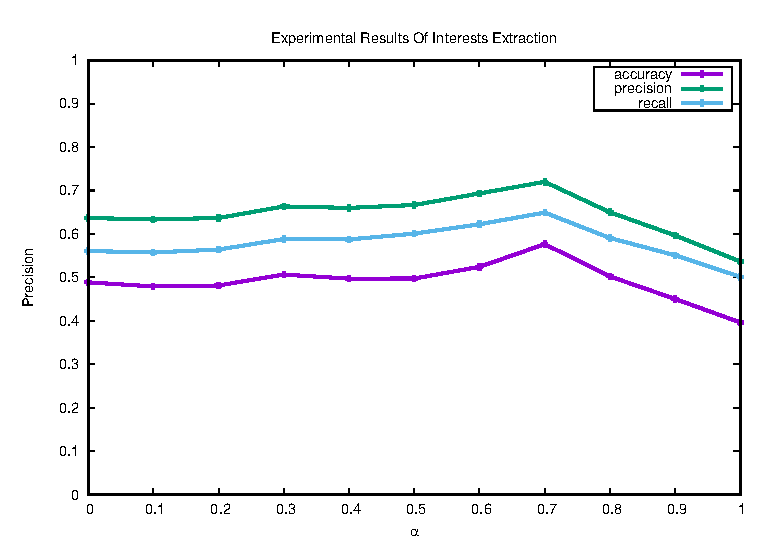
\includegraphics[width=.96\linewidth]{figures/Interests}
\caption{Testing Results with Various $\alpha$ \tbc{}}
\label{fig:fe}
\end{figure}


\textbf{User Clusterer}
%
Fig.\ \ref{fig:uc} depicts the Silhouette Coefficient Values of multiple clustering solutions, with the cluster number from 2 to 10.
Specially, we used different testing datasets, with \textit{Data} containing the overall 43.5K users and \textit{Data1,...,5} contains 10K randomly selected users each.
Except for \textit{Data1}, solutions with 4 clusters sweep.

\begin{figure}[!htb]
\centering
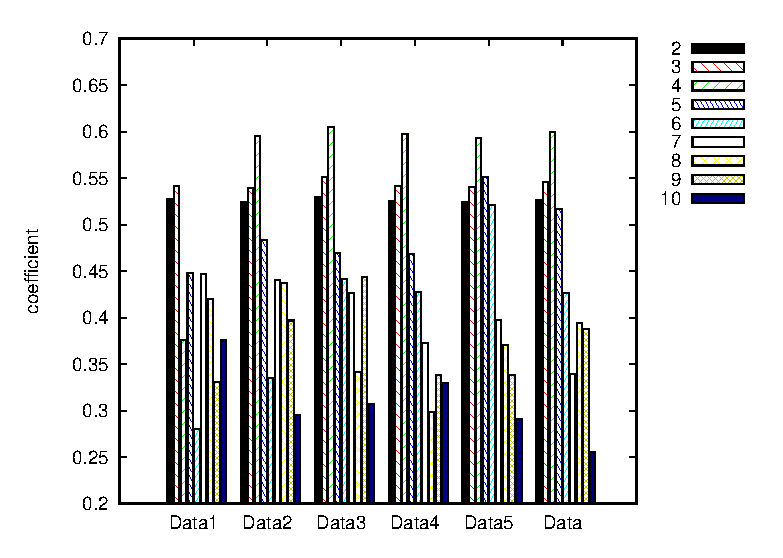
\includegraphics[width=.96\linewidth]{figures/clustering}
\caption{Silhouette Coefficient Values for Various Cluster Numbers over Different Testing Datasets \tbc{}}
\label{fig:uc}
\end{figure}


\textbf{Behavior Modeler}
%
Fig.\ \ref{fig:10} shows the performance of \sys{} against state of the art approach LRC-BQ \refe{}.
We compare the metrics of precision, recall, as well as $F_1$ score.
LRC-BQ \refe{} does not deal with user grouping.
Hence, we not only study the modeling effect per group (i.e., ``Group-One/Two/Three/Four'' with user clustering), but also examine \sys{} versus LRC-BQ \refe{} in the case that all users are in mono group (i.e., ``All-Users'').
The results are interesting in that:
\begin{itemize}
	\item With user clustering, \sys{} performs better than LRC-BQ \refe{} in most cases.
	\item For \sys{}, having user clustering is better than the alternative mono group. Ditto for LRC-BQ \refe{}.
\end{itemize}



\begin{figure}
  \centering
  \subfigure[Precision]{
    \label{fig:10-a} 
    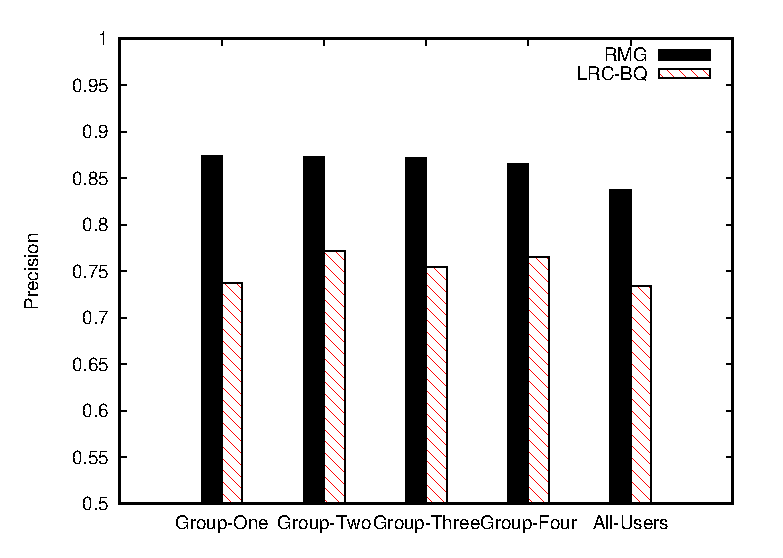
\includegraphics[width=0.4\textwidth]{figures/precision.eps}}
  \hspace{1in}
  \subfigure[Recall]{
    \label{fig:10-b} 
    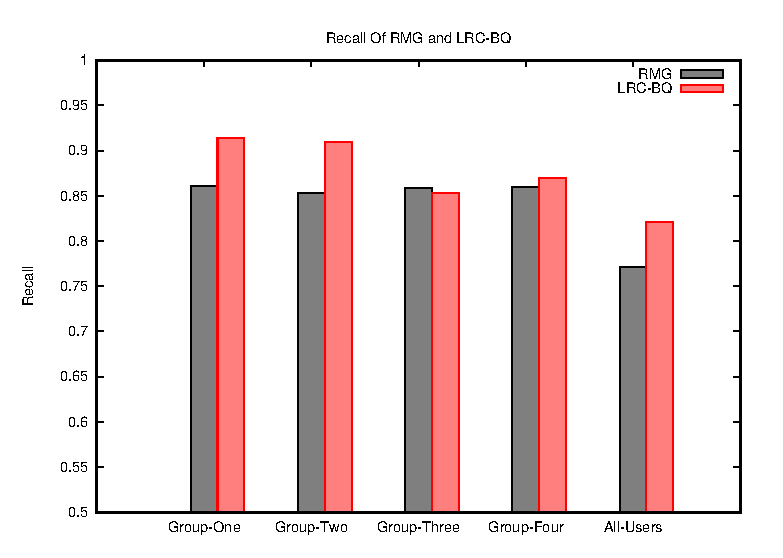
\includegraphics[width=0.4\textwidth]{figures/recall.eps}}
  \hspace{1in}
  \subfigure[$F_1$ Score]{
    \label{fig:10-c} 
    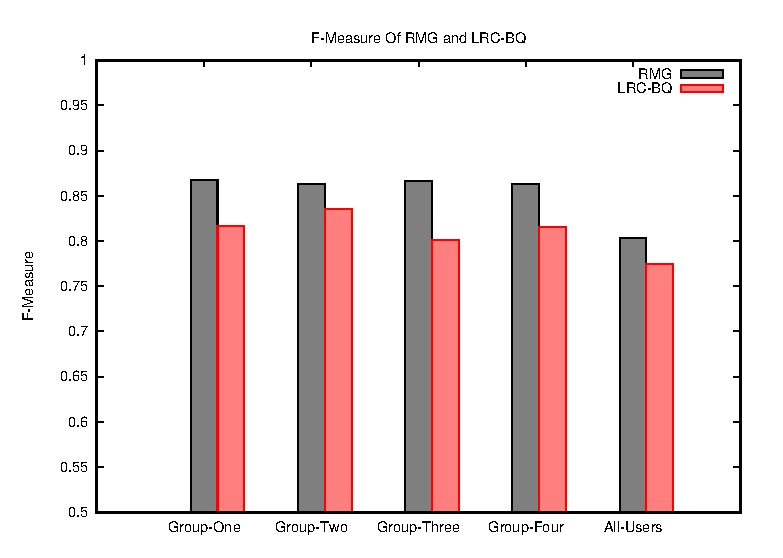
\includegraphics[width=0.4\textwidth]{figures/F-Measure.eps}}
  \caption{Performance of \sys{} Versus LRC-BQ \tbc{}}
  \label{fig:10} 
\end{figure}


Fig.\ \ref{fig:11} explores the performance of \sys{} when using alternative data items for modeling.
By default, \sys{} uses ``UI+II+MI'', i.e., items of users (UI), blogs (MI) and interactions (II).
How about using other combinations of the above item(s)?
As shown in Fig.\ \ref{fig:11}, the default setting wins in most cases.

\begin{figure}
  \centering
  \subfigure[Precision]{
    \label{fig:11-a} 
    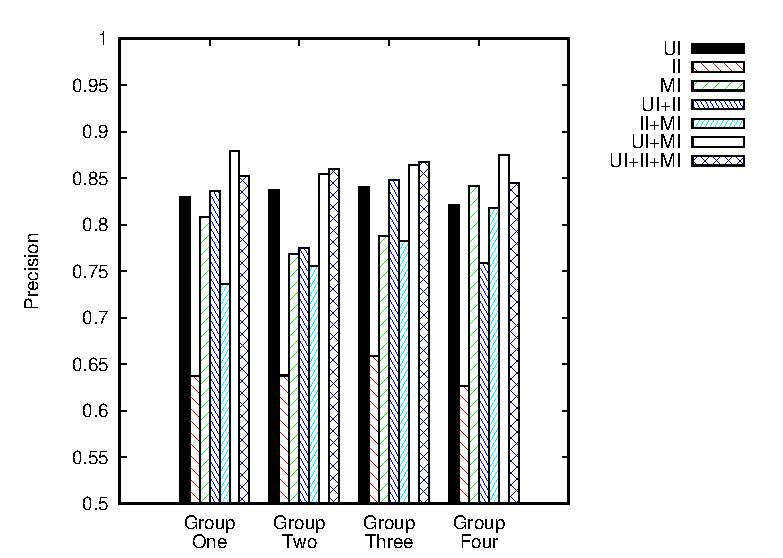
\includegraphics[width=0.4\textwidth]{figures/precisionofdifferentfeatures.eps}}
  \hspace{1in}
  \subfigure[Recall]{
    \label{fig:11-b} 
    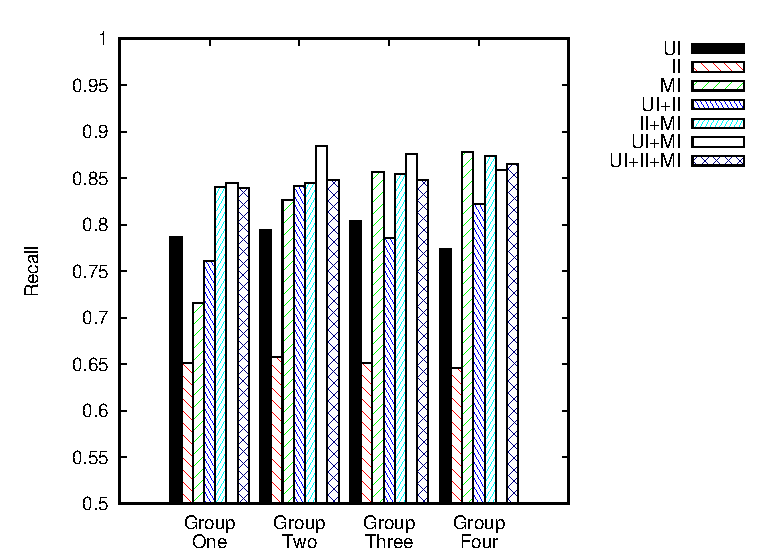
\includegraphics[width=0.4\textwidth]{figures/recallofdifferentfeatures.eps}}
  \hspace{1in}
  \subfigure[$F_1$ Score]{
    \label{fig:11-c} 
    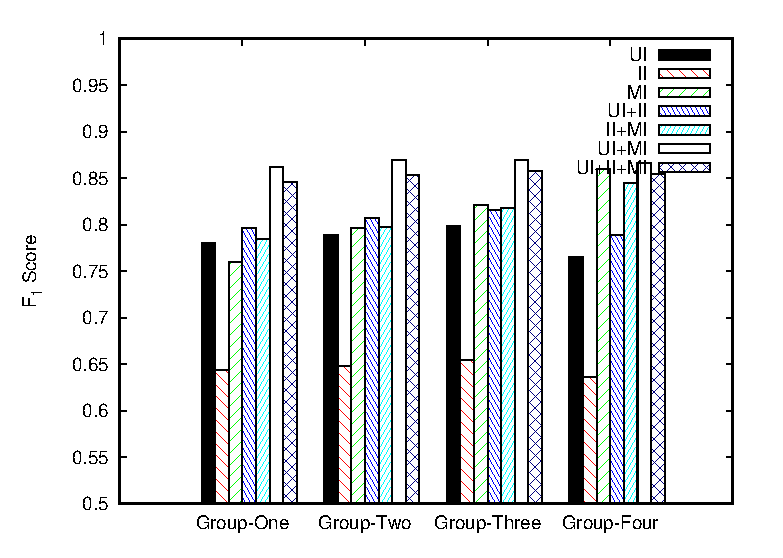
\includegraphics[width=0.4\textwidth]{figures/fmeasureofdifferentfeatures.eps}}
  \caption{\sys{} Performance of Using Various Data Items for Modeling \tbc{}}
  \label{fig:11}
\end{figure}
